% Options for packages loaded elsewhere
\PassOptionsToPackage{unicode}{hyperref}
\PassOptionsToPackage{hyphens}{url}
%
\documentclass[
]{article}
\usepackage{amsmath,amssymb}
\usepackage{lmodern}
\usepackage{iftex}
\ifPDFTeX
  \usepackage[T1]{fontenc}
  \usepackage[utf8]{inputenc}
  \usepackage{textcomp} % provide euro and other symbols
\else % if luatex or xetex
  \usepackage{unicode-math}
  \defaultfontfeatures{Scale=MatchLowercase}
  \defaultfontfeatures[\rmfamily]{Ligatures=TeX,Scale=1}
\fi
% Use upquote if available, for straight quotes in verbatim environments
\IfFileExists{upquote.sty}{\usepackage{upquote}}{}
\IfFileExists{microtype.sty}{% use microtype if available
  \usepackage[]{microtype}
  \UseMicrotypeSet[protrusion]{basicmath} % disable protrusion for tt fonts
}{}
\makeatletter
\@ifundefined{KOMAClassName}{% if non-KOMA class
  \IfFileExists{parskip.sty}{%
    \usepackage{parskip}
  }{% else
    \setlength{\parindent}{0pt}
    \setlength{\parskip}{6pt plus 2pt minus 1pt}}
}{% if KOMA class
  \KOMAoptions{parskip=half}}
\makeatother
\usepackage{xcolor}
\usepackage[margin=1in]{geometry}
\usepackage{longtable,booktabs,array}
\usepackage{calc} % for calculating minipage widths
% Correct order of tables after \paragraph or \subparagraph
\usepackage{etoolbox}
\makeatletter
\patchcmd\longtable{\par}{\if@noskipsec\mbox{}\fi\par}{}{}
\makeatother
% Allow footnotes in longtable head/foot
\IfFileExists{footnotehyper.sty}{\usepackage{footnotehyper}}{\usepackage{footnote}}
\makesavenoteenv{longtable}
\usepackage{graphicx}
\makeatletter
\def\maxwidth{\ifdim\Gin@nat@width>\linewidth\linewidth\else\Gin@nat@width\fi}
\def\maxheight{\ifdim\Gin@nat@height>\textheight\textheight\else\Gin@nat@height\fi}
\makeatother
% Scale images if necessary, so that they will not overflow the page
% margins by default, and it is still possible to overwrite the defaults
% using explicit options in \includegraphics[width, height, ...]{}
\setkeys{Gin}{width=\maxwidth,height=\maxheight,keepaspectratio}
% Set default figure placement to htbp
\makeatletter
\def\fps@figure{htbp}
\makeatother
\setlength{\emergencystretch}{3em} % prevent overfull lines
\providecommand{\tightlist}{%
  \setlength{\itemsep}{0pt}\setlength{\parskip}{0pt}}
\setcounter{secnumdepth}{5}
\newlength{\cslhangindent}
\setlength{\cslhangindent}{1.5em}
\newlength{\csllabelwidth}
\setlength{\csllabelwidth}{3em}
\newlength{\cslentryspacingunit} % times entry-spacing
\setlength{\cslentryspacingunit}{\parskip}
\newenvironment{CSLReferences}[2] % #1 hanging-ident, #2 entry spacing
 {% don't indent paragraphs
  \setlength{\parindent}{0pt}
  % turn on hanging indent if param 1 is 1
  \ifodd #1
  \let\oldpar\par
  \def\par{\hangindent=\cslhangindent\oldpar}
  \fi
  % set entry spacing
  \setlength{\parskip}{#2\cslentryspacingunit}
 }%
 {}
\usepackage{calc}
\newcommand{\CSLBlock}[1]{#1\hfill\break}
\newcommand{\CSLLeftMargin}[1]{\parbox[t]{\csllabelwidth}{#1}}
\newcommand{\CSLRightInline}[1]{\parbox[t]{\linewidth - \csllabelwidth}{#1}\break}
\newcommand{\CSLIndent}[1]{\hspace{\cslhangindent}#1}
\newcommand{\beginappendix}{ \setcounter{table}{0} \renewcommand{\thetable}{A\arabic{table}} \setcounter{figure}{0} \renewcommand{\thefigure}{A\arabic{figure}} }
\usepackage[capposition=top]{floatrow}
\usepackage{placeins}
\usepackage{setspace}
\usepackage{dcolumn}
\usepackage{booktabs}
\usepackage{siunitx}
\usepackage{amsmath}
\usepackage{enumerate}
\usepackage[shortlabels]{enumitem}
\usepackage[hang,flushmargin]{footmisc}
\usepackage{booktabs}
\usepackage{longtable}
\usepackage{array}
\usepackage{multirow}
\usepackage{wrapfig}
\usepackage{float}
\usepackage{colortbl}
\usepackage{pdflscape}
\usepackage{tabu}
\usepackage{threeparttable}
\usepackage{threeparttablex}
\usepackage[normalem]{ulem}
\usepackage{makecell}
\usepackage{xcolor}
\ifLuaTeX
  \usepackage{selnolig}  % disable illegal ligatures
\fi
\IfFileExists{bookmark.sty}{\usepackage{bookmark}}{\usepackage{hyperref}}
\IfFileExists{xurl.sty}{\usepackage{xurl}}{} % add URL line breaks if available
\urlstyle{same} % disable monospaced font for URLs
\hypersetup{
  pdftitle={Pollution, agricultural productivity, and development: Evidence from coal in plants in India},
  pdfauthor={Joshua D. Merfeld},
  hidelinks,
  pdfcreator={LaTeX via pandoc}}

\title{Pollution, agricultural productivity, and development: Evidence from coal in plants in India\footnote{thanks to\ldots{}}}
\author{Joshua D. Merfeld\footnote{KDI School of Public Policy and Management and IZA; \href{mailto:merfeld@kdis.ac.kr}{\nolinkurl{merfeld@kdis.ac.kr}}}}
\date{2023-01-02}

\begin{document}
\maketitle
\begin{abstract}
\noindent abstract\\
\strut \\
\textbf{\textit{Keywords}}:\\
\textbf{\textit{JEL Codes}}:
\end{abstract}

\newpage

\hypertarget{introduction}{%
\section{Introduction}\label{introduction}}

\hypertarget{data-and-methods}{%
\section{Data and methods}\label{data-and-methods}}

\hypertarget{data}{%
\subsection{Data}\label{data}}

SHRUGS: Asher et al. (2021)
Ag productivity: Gangopadhyay et al. (2022)
PM estimates: Hammer et al. (2020)

\hypertarget{methodology}{%
\subsection{Methodology}\label{methodology}}

\hypertarget{results}{%
\section{Results}\label{results}}

\hypertarget{conclusion}{%
\section{Conclusion}\label{conclusion}}

\begin{figure}
\centering
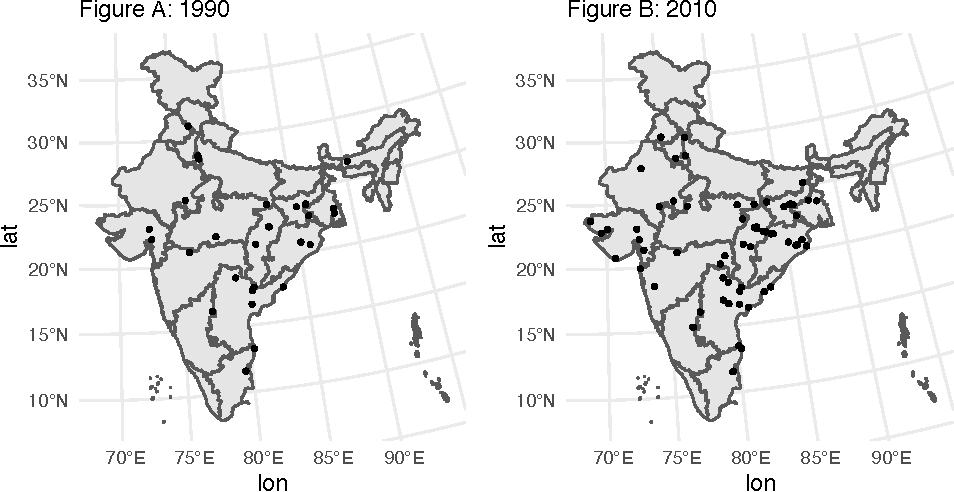
\includegraphics{draft_files/figure-latex/plants-1.pdf}
\caption{\label{fig:plants}Coal plants in India from 1990 to 2010}
\end{figure}

\begin{figure}
\centering
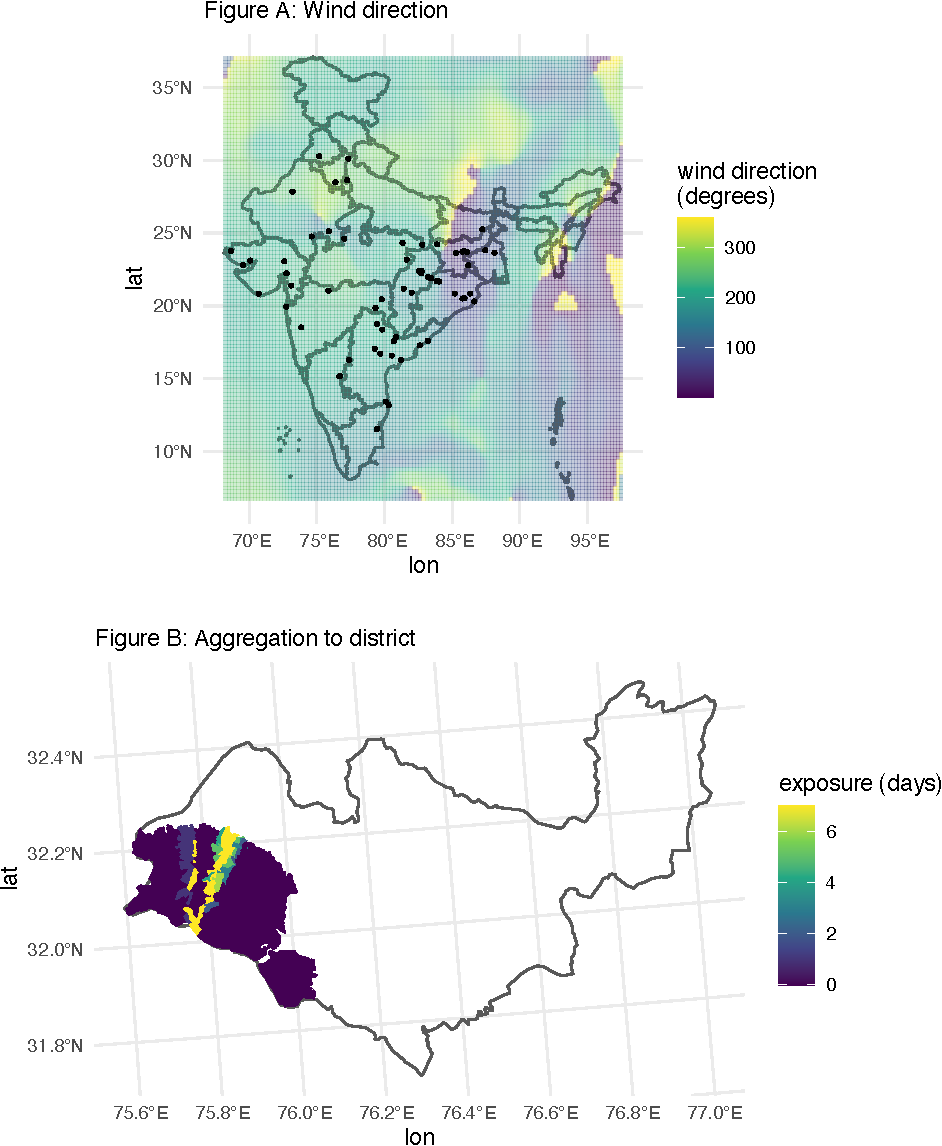
\includegraphics{draft_files/figure-latex/windexample-1.pdf}
\caption{\label{fig:windexample}Wind direction (2010-01-01)}
\end{figure}

\newpage

\begin{table}

\begin{threeparttable}
\caption{\label{tab:pollutiontable}Wind direction and particulate matter}
\centering
\begin{tabular}[t]{>{\raggedright\arraybackslash}p{4cm}>{\centering\arraybackslash}p{2cm}>{\centering\arraybackslash}p{2cm}>{\centering\arraybackslash}p{2cm}>{\centering\arraybackslash}p{2cm}}
\toprule
\multicolumn{1}{c}{ } & \multicolumn{2}{c}{1998-2015} & \multicolumn{2}{c}{2002-2013} \\
\cmidrule(l{3pt}r{3pt}){2-3} \cmidrule(l{3pt}r{3pt}){4-5}
  & (1) & (2) & (3) & (4)\\
\midrule
wind & 0.045*** & 0.040*** & 0.063*** & 0.037***\\
 & (0.004) & (0.006) & (0.005) & (0.007)\\
\textbf{fixed effects:} & \textbf{---------} & \textbf{---------} & \textbf{---------} & \textbf{---------}\\
village & Yes & Yes & Yes & Yes\\
month & Yes & Yes & Yes & Yes\\
\textbf{varying slopes:} & \textbf{---------} & \textbf{---------} & \textbf{---------} & \textbf{---------}\\
month (village) & No & Yes & No & Yes\\
\midrule
observations & 22,345,092 & 22,345,092 & 14,896,728 & 14,896,728\\
\bottomrule
\end{tabular}
\begin{tablenotes}
\small
\item [] Note: Standard errors are in parentheses and are clustered at the village level.
\item [] * p<0.10 ** p<0.05 *** p<0.01
\end{tablenotes}
\end{threeparttable}
\end{table}

\begin{table}

\begin{threeparttable}
\caption{\label{tab:yieldtable}Wind direction and agricultural productivity}
\centering
\begin{tabular}[t]{>{\raggedright\arraybackslash}p{4cm}>{\centering\arraybackslash}p{2cm}>{\centering\arraybackslash}p{2cm}>{\centering\arraybackslash}p{2cm}>{\centering\arraybackslash}p{2cm}}
\toprule
\multicolumn{1}{c}{ } & \multicolumn{2}{c}{all} & \multicolumn{1}{c}{monsoon} & \multicolumn{1}{c}{winter} \\
\cmidrule(l{3pt}r{3pt}){2-3} \cmidrule(l{3pt}r{3pt}){4-4} \cmidrule(l{3pt}r{3pt}){5-5}
  & (1) & (2) & (3) & (4)\\
\midrule
wind & -0.003*** & -0.003*** & -0.002*** & -0.003***\\
 & (0.0002) & (0.0002) & (0.0002) & (0.0003)\\
rain (z) &  & 0.029*** & 0.082*** & 0.016***\\
 &  & (0.0004) & (0.002) & (0.0004)\\
sub-sample & all & all & monsoon & winter\\
\textbf{fixed effects:} & \textbf{---------} & \textbf{---------} & \textbf{---------} & \textbf{---------}\\
village-season & Yes & Yes & No & No\\
year & Yes & Yes & Yes & Yes\\
\midrule
village & No & No & Yes & Yes\\
observations & 2,391,533 & 2,375,337 & 1,259,123 & 1,116,214\\
\bottomrule
\end{tabular}
\begin{tablenotes}
\small
\item [] Note: Standard errors are in parentheses and are clustered at the village level.
\item [] * p<0.10 ** p<0.05 *** p<0.01
\end{tablenotes}
\end{threeparttable}
\end{table}

\begin{table}

\begin{threeparttable}
\caption{\label{tab:yieldtabletwo}Wind direction and agricultural productivity}
\centering
\begin{tabular}[t]{>{\raggedright\arraybackslash}p{4cm}>{\centering\arraybackslash}p{2cm}>{\centering\arraybackslash}p{2cm}>{\centering\arraybackslash}p{2cm}>{\centering\arraybackslash}p{2cm}}
\toprule
\multicolumn{1}{c}{ } & \multicolumn{2}{c}{all} & \multicolumn{1}{c}{monsoon} & \multicolumn{1}{c}{winter} \\
\cmidrule(l{3pt}r{3pt}){2-3} \cmidrule(l{3pt}r{3pt}){4-4} \cmidrule(l{3pt}r{3pt}){5-5}
  & (1) & (2) & (3) & (4)\\
\midrule
pm25 & -0.021*** & -0.020*** & -0.013*** & -0.024***\\
 & (0.001) & (0.002) & (0.001) & (0.003)\\
rain (z) &  & 0.004** & 0.086*** & -0.016***\\
 &  & (0.002) & (0.002) & (0.004)\\
sub-sample & all & all & monsoon & winter\\
\textbf{fixed effects:} & \textbf{---------} & \textbf{---------} & \textbf{---------} & \textbf{---------}\\
village-season & Yes & Yes & No & No\\
year & Yes & Yes & Yes & Yes\\
village & No & No & Yes & Yes\\
\midrule
observations & 2,391,533 & 2,375,337 & 1,259,123 & 1,116,214\\
\midrule
\textbf{first stage:} & \textbf{} & \textbf{} & \textbf{} & \textbf{}\\
wind & 0.143*** & 0.126*** & 0.155*** & 0.105***\\
 & (0.003) & (0.003) & (0.003) & (0.004)\\
rain (z) &  & -1.23*** & 0.301*** & -1.36***\\
 &  & (0.010) & (0.015) & (0.009)\\
\bottomrule
\end{tabular}
\begin{tablenotes}
\small
\item [] Note: Standard errors are in parentheses and are clustered at the village level.
\item [] * p<0.10 ** p<0.05 *** p<0.01
\end{tablenotes}
\end{threeparttable}
\end{table}

\begin{table}

\begin{threeparttable}
\caption{\label{tab:labortable}Wind direction and labor allocation}
\centering
\begin{tabular}[t]{>{\raggedright\arraybackslash}p{4cm}>{\centering\arraybackslash}p{2cm}>{\centering\arraybackslash}p{2cm}>{\centering\arraybackslash}p{2cm}}
\toprule
  & (1) & (2) & (3)\\
\midrule
wind & -0.028* & -0.035** & -0.027*\\
 & (0.015) & (0.015) & (0.015)\\
controls & No & Yes & Yes\\
\textbf{fixed effects:} & \textbf{-------} & \textbf{--------} & \textbf{-------}\\
district & Yes & Yes & Yes\\
year & Yes & Yes & Yes\\
\textbf{varying slopes:} & \textbf{-------} & \textbf{--------} & \textbf{-------}\\
year (district) & No & No & Yes\\
\midrule
observations & 899,045 & 898,856 & 898,856\\
\bottomrule
\end{tabular}
\begin{tablenotes}
\small
\item [] Note: Standard errors are in parentheses and are clustered at the village level.
\item [] * p<0.10 ** p<0.05 *** p<0.01
\end{tablenotes}
\end{threeparttable}
\end{table}

\FloatBarrier
\newpage

\hypertarget{references}{%
\section*{References}\label{references}}
\addcontentsline{toc}{section}{References}

\hypertarget{refs}{}
\begin{CSLReferences}{1}{0}
\leavevmode\vadjust pre{\hypertarget{ref-almn2021}{}}%
Asher, Sam, Tobias Lunt, Ryu Matsuura, and Paul Novosad. 2021. {``{Development Research at High Geographic Resolution: An Analysis of Night Lights, Firms, and Poverty in India using the SHRUG Open Data Platform}.''} \emph{{The World Bank Economic Review}}.

\leavevmode\vadjust pre{\hypertarget{ref-gangopadhyay2022new}{}}%
Gangopadhyay, Prasun K, Paresh B Shirsath, Vinay K Dadhwal, and Pramod K Aggarwal. 2022. {``{A new two-decade (2001--2019) high-resolution agricultural primary productivity dataset for India}.''} \emph{{Scientific Data}} 9 (1): 1--12.

\leavevmode\vadjust pre{\hypertarget{ref-hammer2020global}{}}%
Hammer, Melanie S, Aaron van Donkelaar, Chi Li, Alexei Lyapustin, Andrew M Sayer, N Christina Hsu, Robert C Levy, et al. 2020. {``Global Estimates and Long-Term Trends of Fine Particulate Matter Concentrations (1998--2018).''} \emph{{Environmental Science \& Technology}} 54 (13): 7879--90.

\end{CSLReferences}

\FloatBarrier

\beginappendix

\newpage

\hypertarget{appendix-a}{%
\section*{Appendix A}\label{appendix-a}}
\addcontentsline{toc}{section}{Appendix A}

\FloatBarrier
\singlespacing

\begin{table}

\caption{\label{tab:pmeffects}Particulate matter and agricultural productivity}
\centering
\begin{tabular}[t]{>{\raggedright\arraybackslash}p{4cm}>{\centering\arraybackslash}p{2cm}>{\centering\arraybackslash}p{2cm}>{\centering\arraybackslash}p{2cm}>{\centering\arraybackslash}p{2cm}}
\toprule
\multicolumn{1}{c}{ } & \multicolumn{2}{c}{all} & \multicolumn{1}{c}{monsoon} & \multicolumn{1}{c}{winter} \\
\cmidrule(l{3pt}r{3pt}){2-3} \cmidrule(l{3pt}r{3pt}){4-4} \cmidrule(l{3pt}r{3pt}){5-5}
  & (1) & (2) & (3) & (4)\\
\midrule
particulate matter & 0.045 & 0.501*** & 2.05*** & 0.472***\\
(PM 2.5, '000s) & (0.031) & (0.031) & (0.099) & (0.037)\\
rain (z) &  & 0.030*** & 0.083*** & 0.017***\\
 &  & (0.0004) & (0.002) & (0.0004)\\
sub-sample & all & all & monsoon & winter\\
\textbf{fixed effects:} & \textbf{-------} & \textbf{---------} & \textbf{---------} & \textbf{---------}\\
village-season & Yes & Yes & No & No\\
year & Yes & Yes & Yes & Yes\\
village & No & No & Yes & Yes\\
\midrule
observations & 2,391,533 & 2,375,337 & 1,259,123 & 1,116,214\\
\midrule
\bottomrule
\multicolumn{5}{l}{\textsuperscript{} Note: Standard errors are in parentheses and are clustered at the village}\\
\multicolumn{5}{l}{level.}\\
\multicolumn{5}{l}{\textsuperscript{} * p<0.10 ** p<0.05 *** p<0.01}\\
\end{tabular}
\end{table}

\end{document}
